\documentclass[tikz,border=10pt]{standalone}
\usepackage{tikz}

\begin{document}

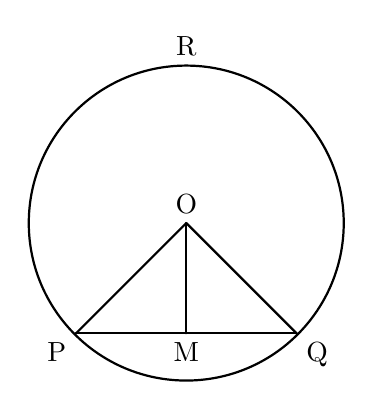
\begin{tikzpicture}[scale=1, line cap=round, line join=round]

% Center
\coordinate (O) at (0,0);

% Draw Circle
\draw[thick] (O) circle (2);

% Points
\coordinate (P) at (-1.4, -1.4);
\coordinate (Q) at (1.4, -1.4);
\coordinate (M) at (0, -1.4);
\coordinate (R) at (0, 2);

% Segments
\draw[thick] (P) -- (Q);
\draw[thick] (O) -- (P);
\draw[thick] (O) -- (Q);
\draw[thick] (O) -- (M);

% Labels
\node[above] at (O) {O};
\node[above] at (R) {R};
\node[below left] at (P) {P};
\node[below right] at (Q) {Q};
\node[below] at (M) {M};

\end{tikzpicture}

\end{document}
